\chapter{Progettazione e implementazione} %\label{1cap:spinta_laterale}
% [titolo ridotto se non ci dovesse stare] {titolo completo}
%

\begin{citazione}
In questo capitolo viene mostrato passo passo un procedimento guida alla realizazzione di un motore scacchistico
\end{citazione}

\newpage
\section{Prefazione} %\label{1sec:scopo}
Lo sviluppo di un motore scacchistico è fortemente influenzato dalle scelte progettuali,
una di queste è il linguaggio di programmazione che si vuole utilizzare,
le prestazioni di un motore possono essere fortemente influenzate dalla natura del linguaggio di 
programmazione, in particolare l'utilizzo di un linguaggio interpretato e non compilato può impattare
notevolmente sulla velocità con la quale il nostro motore è in grado di elaborare le milioni di 
posizioni con le quali dovrà avere a che fare in una singola partita.
Tutti gli esempi di codice all'interno di questa tesi saranno scritti nel linguaggio C, si consiglia
quindi di avere almeno una minima familiarità con tale linguaggio.Si segnalano comunque diversi 
tool  per il linguaggio python per chi volesse approcciarsi a questo mondo utilizzando un
linguaggio più beginner friendly  quali:
\begin{itemize}
	\item \textbf{python-chess}: una libreria di python che contiene funzioni di libreria per la rappresentazione 
          di scacchiera e pezzi e per la generazione e validazione delle mosse,utile se ci si vuole concentrare
          esclusivamente sulla parte di ricerca e di valutazione  di un motore scacchistico.
	\item \textbf{Sunfish}: un motore scacchistico per principianti scritto nel linguaggio python che
           in sole 111 linee di codice illustra ,in maniera semplificata, l'implementazione della 
           gran parte dei concetti  chiave di un motore scacchistico.

\end{itemize}


\section{Rappresentazione della scacchiera e dei pezzi} %\label{1sec:scopo}
Il primo passo dello sviluppo di un motore scacchistico è decidere come si vuole rappresentare 
la scacchiera , si tratta di una scelta fondamentale,non solo perché in seguito ci permetterà
di testare le funzioni che andremo a implementare, ma anche perché è nella scacchiera che ,generalmente,
viene conservato lo stato generale della partita.\footnote{per stato di una partita si intendono informazioni come
informazioni su chi ha diritto di muovere, i permessi di arrocco,lo stato della regola delle 50 mosse etc} 
Inoltre il tipo di codifica può influenzare la rapidità
e la facilità col quale possiamo accedere alle informazioni sullo stato corrente dei pezzi 
e come vedremo in seguito è in grado di influenzare funzioni come la generazione delle mosse.
Non è raro per motori scacchistici particolarmente complessi l'utilizzo di più tipi di board in base
al tipo di informazione da conservare e all'utilizzo che se ne vuole fare.
Per la rappresentazione di una scacchiera sono chiaramente possibili moltissime scelte, di seguito
verranno illustrate alcune tra le più popolari ed utilizzate.

\subsection{Rappresentazione Pezzocentrica}
Si definisce rappresentazione pezzocentrica, un qualsiasi tipo di rappresentazione della scacchiera che mantiene liste
array o set dei pezzi attualmente presenti sulla scacchiera con annesse le informazioni sulle caselle da essi occupate.
Le rappresentazioni più comuni sono: 
\subsubsection{Piece-Lists}
liste o array di ogni pezzo sulla scacchiera,ogni elemento della lista o dell'array associa un pezzo
alla casella che esso occupa .le caratteristiche di ogni pezzo (colore,tipo etc) 
 possono essere associate all'indice dell'array in cui si trovano o essere presenti in ulteriori array 
 o liste esterne. \emph{un'implementazione pratica di una Piece-List verrà mostrata in seguito all'interno
 di questo capitolo}
 
\subsubsection{Bitboards} 
Una Bitboard è una struttura dati specifica per i giochi da tavolo,
si tratta in sostanza  di una struttura dati in grado di immagazzinare lo stato di ogni casella della 
scacchiera all'interno di una parola \footnote{Una parola è un gruppo di bit di una determinata dimensione che sono gestiti come unità dal set di istruzioni o dall'hardware di un processore} di 64 bit.
Vediamo un esempio pratico, immaginiamo di avere una scacchiera che si trova nello stato di default di inizio
partita:\\
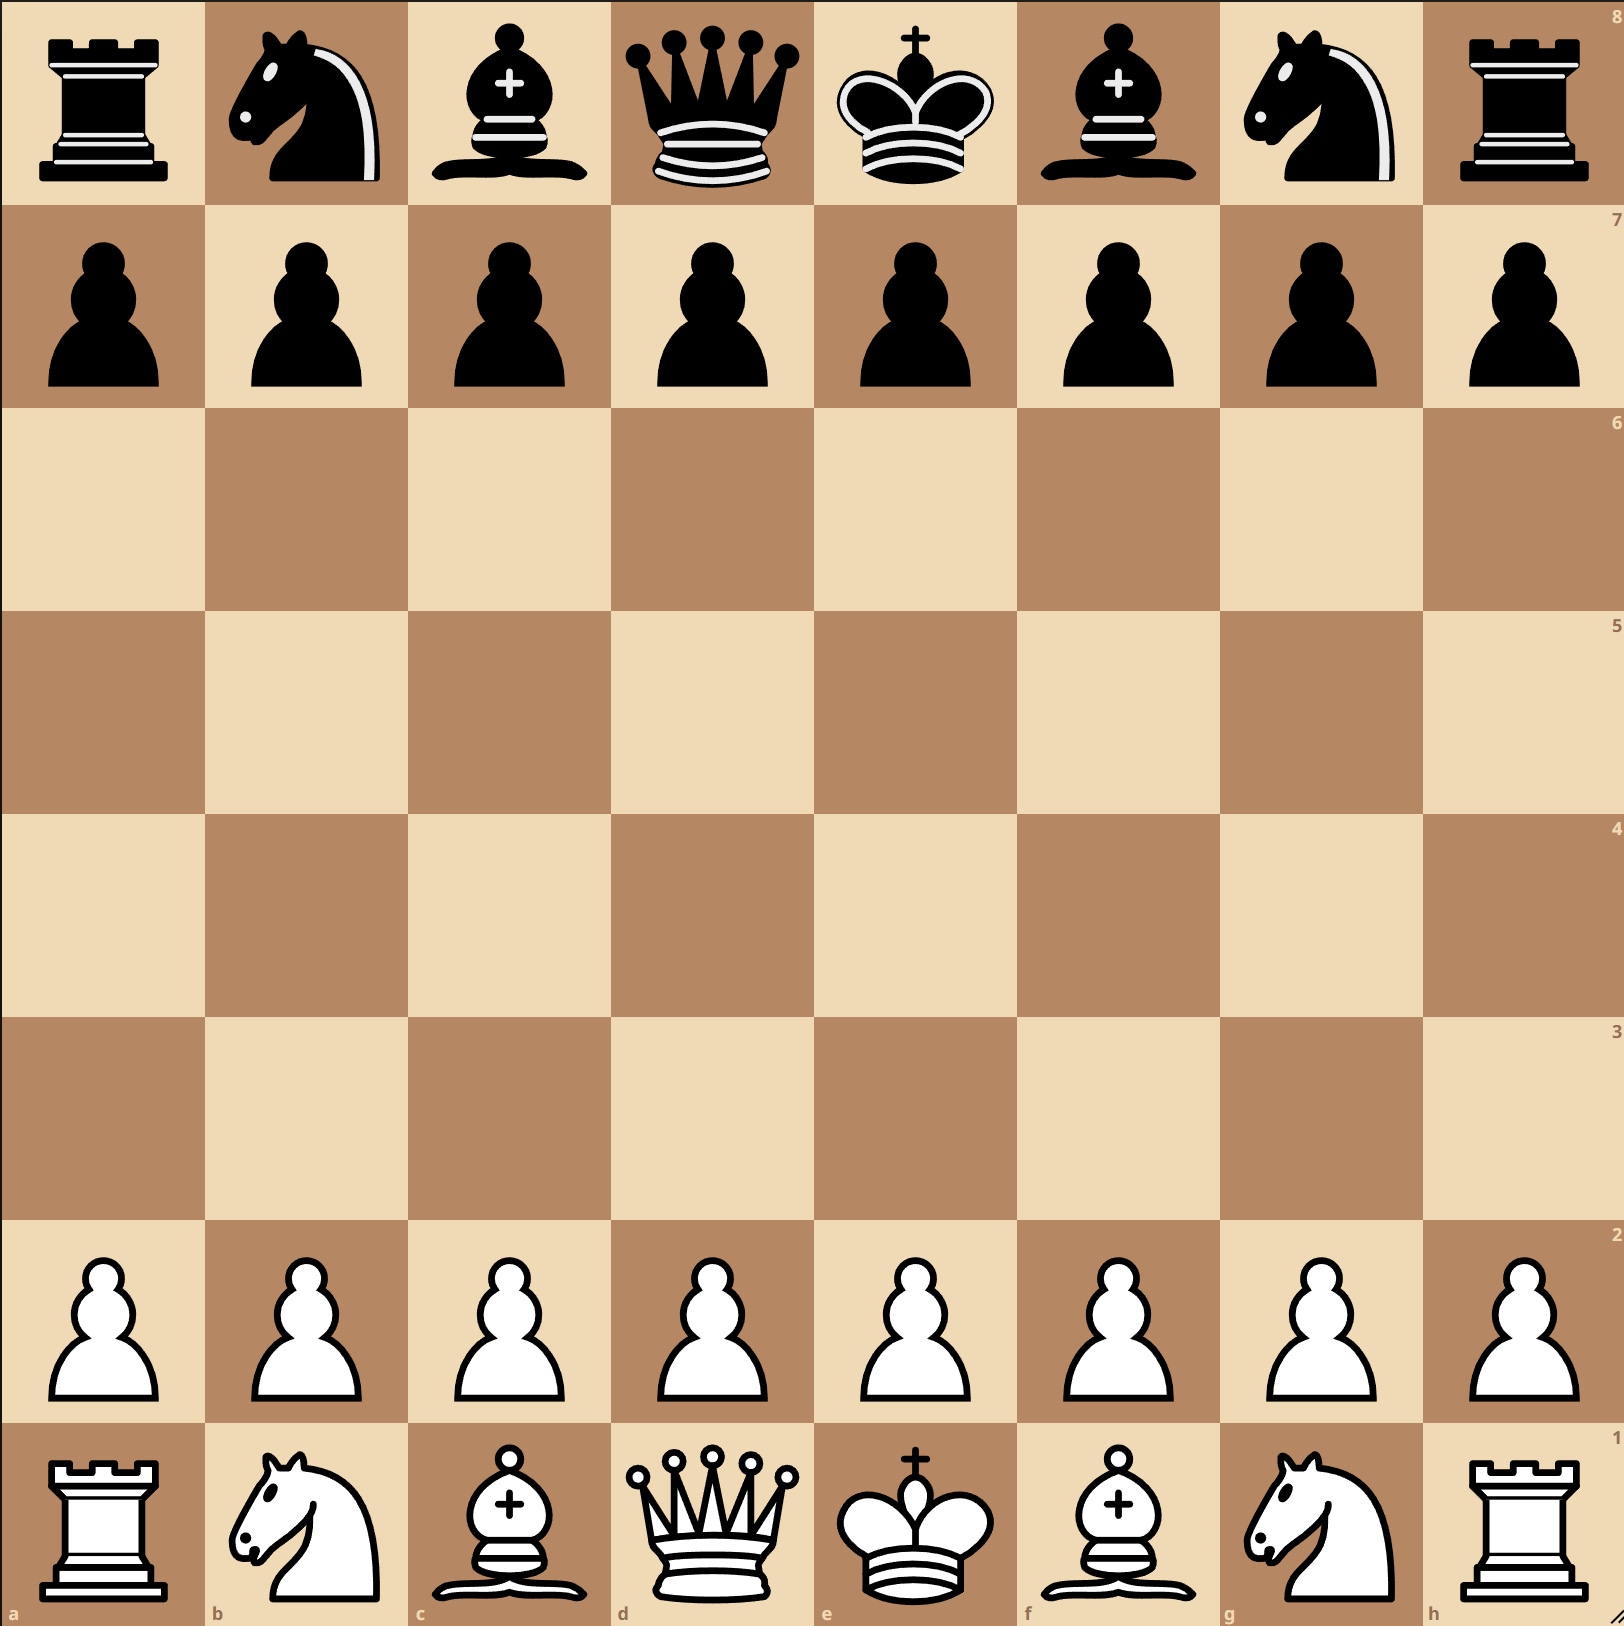
\includegraphics[scale=0.5] {scacchiera.png}\\
Una bitboard tipica è quella che ci permette di sapere in quali caselle è presente un pedone
nero,per costruirla, operando casella per casella, ci poniamo una domanda "in questa casella
è presente un pedone nero?" se si allora quella casella viene marcata con un 1 , altrimenti viene
marcata con uno 0, il risultato di questa traduzione diventa in questo caso:\\
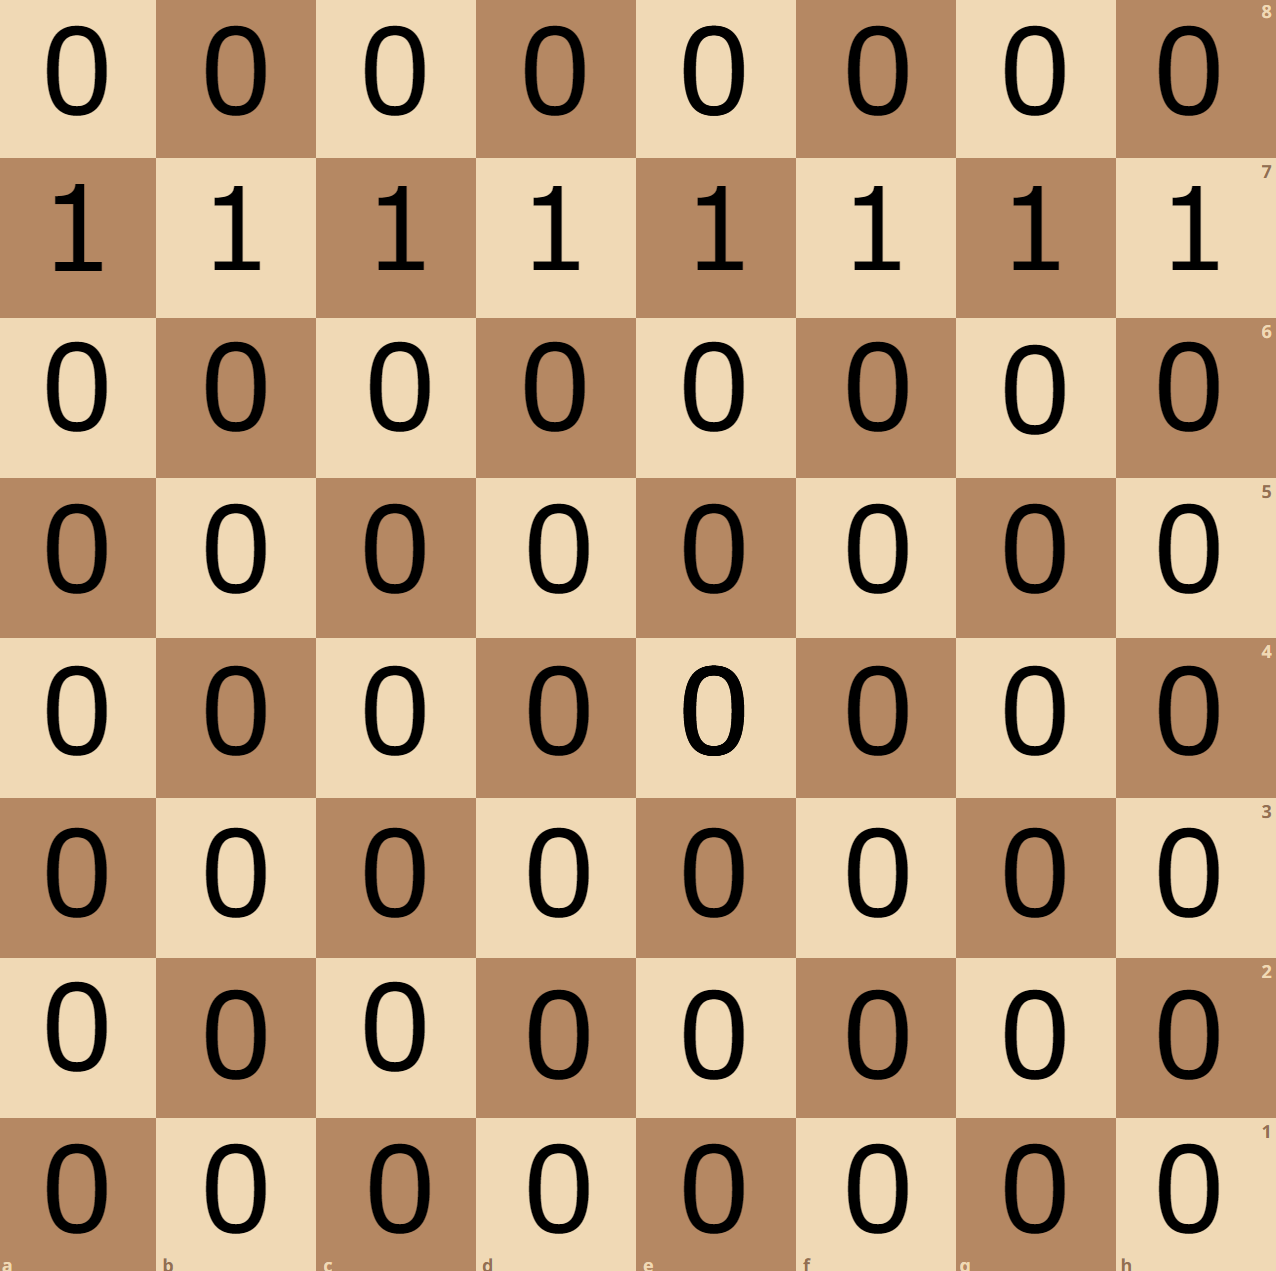
\includegraphics[scale=0.3] {bitboard.png}
\subsubsection{Piece-Sets}
rappresentazione con set con un bit per ogni pezzo dentro una parola a 32 bit o 2 parole a 16 bit (una per lato) 
i Piece-sets hanno  delle somiglianze con le bitboards, ma ogni  bit del set non è   direttamente correlato ad una casella, 
ma ad un indice  dentro ad una  piece-list. Spesso la bit-position di un  piece-set  implica 
 , di che tipo e colore il pezzo è. - mentre le  bitboards solitamente mantengono set distinti  
 per pezzi diversi.


\subsection{Rappresentazione Casellocentrica}
\subsubsection{Mailbox}
\subsubsection{8x8 Board}
\subsubsection{10x12 Board}
\subsubsection{Vector Attacks}
\subsubsection{0x88}





\section{Move Generation} %\label{1sec:scopo}


\section{Ricerca} %\label{1sec:scopo}

\section{Valutazione} %\label{1sec:scopo}

\section{libro delle aperture,Tablebases} %\label{1sec:scopo}

